% Standalone TikZ figure: Exploration vs Exploitation in Bayesian Optimization
% For Chapter 3: Reinforcement Learning for Parameter Optimization
\documentclass[tikz,border=10pt]{standalone}
\usepackage{tikz}
\usepackage{amsmath}
\usetikzlibrary{arrows.meta, positioning, shapes.geometric, fit, backgrounds, calc, patterns, decorations.pathreplacing, shadings}

\begin{document}
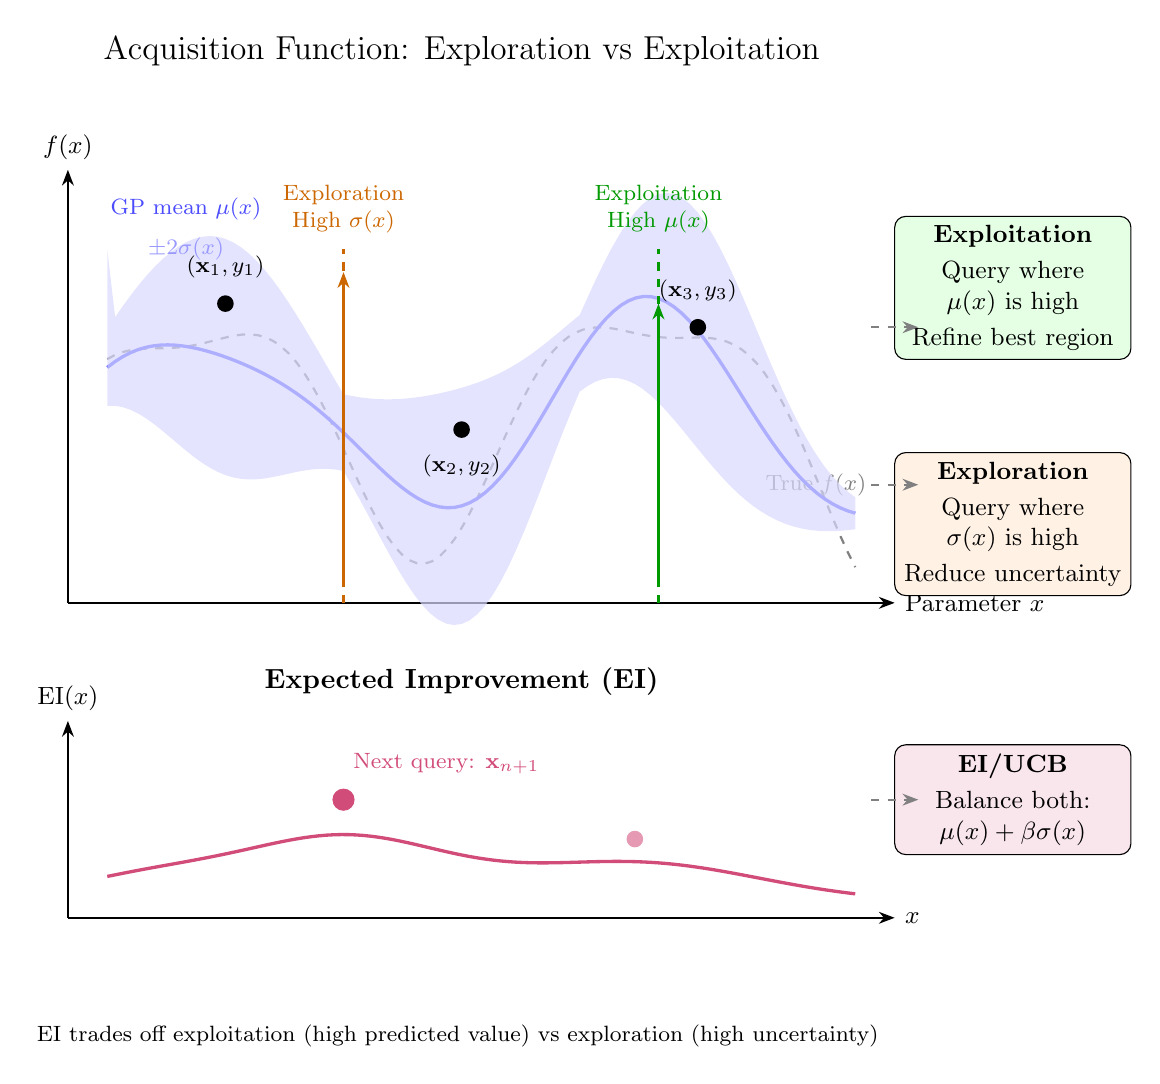
\begin{tikzpicture}[
    every node/.style={font=\small},
    arrow/.style={-{Stealth[length=2mm]}, thick},
    label/.style={font=\footnotesize},
    title/.style={font=\bfseries}
]

% ============ GAUSSIAN PROCESS SURROGATE ============
\node[title, font=\large] at (5, 7) {Acquisition Function: Exploration vs Exploitation};

% Axes
\draw[arrow] (0, 0) -- (10.5, 0) node[right] {Parameter $x$};
\draw[arrow] (0, 0) -- (0, 5.5) node[above] {$f(x)$};

% True function (hidden, shown as dashed for reference)
\draw[gray, dashed, thick, domain=0.5:10, samples=100] plot (\x, {2.5 + 1.5*sin(60*\x) + 0.5*cos(120*\x) - 0.02*(\x-5)*(\x-5)});
\node[label, text=gray] at (9.5, 1.5) {True $f(x)$};

% GP mean function
\draw[blue!70, very thick, domain=0.5:10, samples=100] plot (\x, {2.5 + 1.2*sin(60*\x) + 0.3*cos(100*\x) - 0.015*(\x-5)*(\x-5)});

% Uncertainty band (shaded region)
\fill[blue!15, opacity=0.7]
    (0.5, {2.5 + 1.2*sin(60*0.5) + 0.3*cos(100*0.5) - 0.015*(0.5-5)*(0.5-5) + 1.5})
    \foreach \x in {0.6, 0.7, ..., 10} {
        -- (\x, {2.5 + 1.2*sin(60*\x) + 0.3*cos(100*\x) - 0.015*(\x-5)*(\x-5) + 1.5*exp(-0.5*pow(min(min(abs(\x-2),abs(\x-5)),abs(\x-8)),2))})
    }
    -- (10, {2.5 + 1.2*sin(60*10) + 0.3*cos(100*10) - 0.015*(10-5)*(10-5) - 1.5*exp(-0.5*pow(min(min(abs(10-2),abs(10-5)),abs(10-8)),2))})
    \foreach \x in {10, 9.9, 9.8, ..., 0.5} {
        -- (\x, {2.5 + 1.2*sin(60*\x) + 0.3*cos(100*\x) - 0.015*(\x-5)*(\x-5) - 1.5*exp(-0.5*pow(min(min(abs(\x-2),abs(\x-5)),abs(\x-8)),2))})
    }
    -- cycle;

% Observed data points
\fill[black] (2, 3.8) circle (3pt);
\fill[black] (5, 2.2) circle (3pt);
\fill[black] (8, 3.5) circle (3pt);

% Labels for observed points
\node[label, above] at (2, 4.0) {$(\mathbf{x}_1, y_1)$};
\node[label, below] at (5, 2.0) {$(\mathbf{x}_2, y_2)$};
\node[label, above] at (8, 3.7) {$(\mathbf{x}_3, y_3)$};

% Legend for GP
\node[label, text=blue!70] at (1.5, 5) {GP mean $\mu(x)$};
\node[label, text=blue!40] at (1.5, 4.5) {$\pm 2\sigma(x)$};

% ============ EXPLOITATION REGION ============
\draw[green!60!black, very thick, dashed] (7.5, 0) -- (7.5, 4.5);
\node[label, text=green!60!black, align=center] at (7.5, 5) {Exploitation\\High $\mu(x)$};
\draw[arrow, green!60!black, very thick] (7.5, 0.2) -- (7.5, 3.8);

% ============ EXPLORATION REGION ============
\draw[orange!80!black, very thick, dashed] (3.5, 0) -- (3.5, 4.5);
\node[label, text=orange!80!black, align=center] at (3.5, 5) {Exploration\\High $\sigma(x)$};
\draw[arrow, orange!80!black, very thick] (3.5, 0.2) -- (3.5, 4.2);

% ============ ACQUISITION FUNCTION SUBPLOT ============
\node[title] at (5, -1) {Expected Improvement (EI)};

% Axes for EI
\draw[arrow] (0, -4) -- (10.5, -4) node[right] {$x$};
\draw[arrow] (0, -4) -- (0, -1.5) node[above] {EI$(x)$};

% EI curve (combination of mean and uncertainty)
\draw[purple!70, very thick, domain=0.5:10, samples=100] plot (\x, {-3.8 + 0.8*exp(-0.3*pow(\x-3.5,2)) + 0.5*exp(-0.2*pow(\x-7.2,2)) + 0.3*exp(-0.4*pow(\x-1,2))});

% Highlight optimal next query point
\fill[purple!70] (3.5, -2.5) circle (4pt);
\node[label, text=purple!70, above right] at (3.5, -2.3) {Next query: $\mathbf{x}_{n+1}$};

% Secondary peak
\fill[purple!40] (7.2, -3.0) circle (3pt);

% ============ DECISION BOXES ============
\node[draw, rounded corners, fill=green!10, minimum width=3cm, align=center] at (12, 4) {
    \textbf{Exploitation}\\[2pt]
    Query where\\
    $\mu(x)$ is high\\[2pt]
    Refine best region
};

\node[draw, rounded corners, fill=orange!10, minimum width=3cm, align=center] at (12, 1) {
    \textbf{Exploration}\\[2pt]
    Query where\\
    $\sigma(x)$ is high\\[2pt]
    Reduce uncertainty
};

\node[draw, rounded corners, fill=purple!10, minimum width=3cm, align=center] at (12, -2.5) {
    \textbf{EI/UCB}\\[2pt]
    Balance both:\\
    $\mu(x) + \beta\sigma(x)$
};

% Arrows connecting
\draw[arrow, gray, dashed] (10.2, 3.5) -- (10.8, 3.5);
\draw[arrow, gray, dashed] (10.2, 1.5) -- (10.8, 1.5);
\draw[arrow, gray, dashed] (10.2, -2.5) -- (10.8, -2.5);

% ============ ANNOTATIONS ============
\node[label, align=left] at (5, -5.5) {
    EI trades off exploitation (high predicted value) vs exploration (high uncertainty)
};

\end{tikzpicture}
\end{document}
